\documentclass[10pt]{beamer}

\usetheme[progressbar=frametitle]{metropolis}
\usepackage{mathtools}
\usepackage{amsmath}
\usepackage{booktabs}
\usepackage[scale=2]{ccicons}

\usepackage{pgfplots}
\usepgfplotslibrary{dateplot}
\usepackage{graphicx}
\graphicspath{}
 

\DeclareMathOperator*{\argmaxA}{arg\,max} % Jan Hlavacek
\DeclareMathOperator*{\argminB}{argmin}   % Jan Hlavacek
\DeclareMathOperator*{\argminC}{\arg\min}   % rbp

\newcommand{\argminD}{\arg\!\min} % AlfC

\newcommand{\argminE}{\mathop{\mathrm{argmin}}}          % ASdeL
\newcommand{\argminF}{\mathop{\mathrm{argmin}}\limits}   % ASdeL

\usepackage{xspace}
\newcommand{\themename}{\textbf{\textsc{metropolis}}\xspace}

\title{
Identificação Automática de Espécies de Pássaros 
}
\subtitle{}
\date{\today}
\author{Felipe Felix $(f^2)$}
\institute{IME-USP}

\begin{document}

\maketitle

%\begin{frame}{Table of contents}
%  \setbeamertemplate{section in toc}[sections numbered]
%  \tableofcontents[hideallsubsections]
%\end{frame}

%\section{Introdução}

\begin{frame}[fragile]{Introdução}

Processo de classificação:
\begin{enumerate}
\item O canto do pássaro é gravado no campo;
\item O áudio é pré-processado para melhorar a qualidade do sinal;
\item Extrai-se as características do sinal de áudio;
\item Então, utiliza-se as características em algoritmos
de aprendizagem de máquina para produzir um procedimento de decisão 
para novas gravações.
\end{enumerate}
\begin{itemize}
\item \textit{Framework} clássico de aprendizagem supervisionada.
\end{itemize}
\end{frame}



\begin{frame}[fragile]{Formulação probabilística do problema}
\begin{itemize}
\item Dado um sinal de áudio $\mathcal{S}$ contendo um canto de pássaro, 
precisamos escolher uma classe $\hat{b}$ de um conjunto finito de classes
$\mathcal{B}$ que melhor representa a espécie que produz aquele canto.
\item Seja $\bar{X}$ o vetor de características derivado de $\mathcal{S}$,
queremos determinar a classe $\hat{b} \in \mathcal{B}$ tal que:
\begin{equation}
\hat{b} = \argmaxA_{b \in \mathcal{B}} P(b \mid \bar{X}) 
\end{equation}


\end{itemize}
\end{frame}

\begin{frame}{Formulação probabilística do problema}
\begin{itemize}
\item Pelo Teorema de Bayes:

\begin{equation}
\hat{b} = \argmaxA_{b \in \mathcal{B}} \frac{P(\hat{X} \mid b)  P(b)}{P(\hat{X})}
\end{equation}

\item Sabemos que $\sum_{b \in \mathcal{B}}P(b \mid \bar{X}) = 1$. Então
$P(\bar{X}) = \sum_{b \in \mathcal{B}} P(\bar{X} \mid b)P(b)$.

\item Então a probabilidade desejada é:
\begin{equation}
P(b \mid \bar{X}) = \frac{P(\bar{X} \mid b)P(b)}{\sum_{b \in \mathcal{B}} P(\bar{X} \mid b)P(b)}
\end{equation}

\item Como o denominador da Eq. 3 é o mesmo para todas as classes, a solução é dada
pela classe
\begin{equation}
\hat{b} = \argmaxA_{b \in \mathcal{B}}P(\hat{X} \mid b)P(b)
\end{equation}

\end{itemize}
\end{frame}

\begin{frame}[fragile]{Dataset}
\begin{itemize}
\item Espécies de pássaros de uma região geográfica comum: Sul da Costa Atlântica
Brasileira.
\item \textit{Dataset} principal: 1619 gravações de 73 espécies de pássaros.
\item Gravações baixadas do Xeno-Canto\footnote{http://www.xeno-canto.org/}.
\item \textit{Dataset} secundário: derivado do principal. As gravações do \textit{dataset}
principal foram divididas em \textit{pulsos}.
\item Pulso: Intervalo pequeno de som com altas amplitudes.

\end{itemize}
\end{frame}


\begin{frame}[fragile]{Extração de características}
\begin{itemize}
\item \textit{Framework} Marsyas\footnote{http://marsyas.info/doc/sourceDoc/html/index.html};
\item 50+ \textit{features};
\end{itemize}
\end{frame}


\begin{frame}[fragile]{Experimentos}
\begin{itemize}
\item \textit{5-fold cross-validation}: os resultados são obtidos de 5 repetições
aleatórias;
\item Os experimentos variam em três dimensões: sinal completo ou uso dos pulsos;
uso de diferentes classificadores; número de classes.
\end{itemize}
\end{frame}

\begin{frame}[fragile]{Resultados}
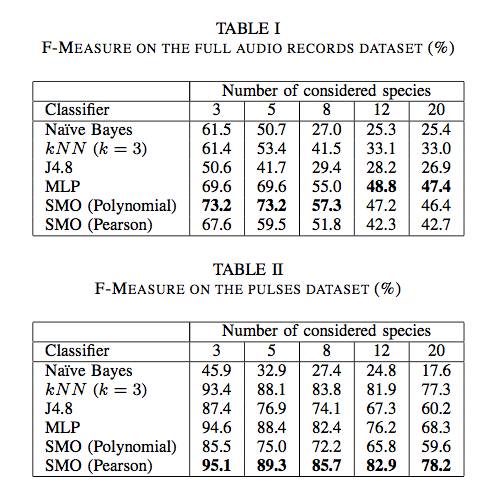
\includegraphics[width=\textwidth, height=8cm]{table12}
\end{frame}


\begin{frame}[fragile]{Resultados}
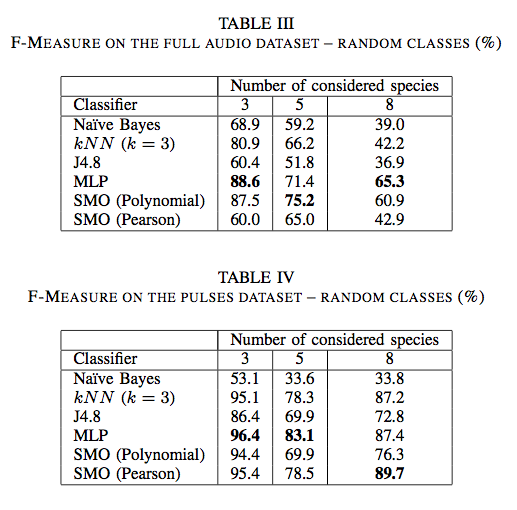
\includegraphics[width=\textwidth, height=8cm]{table34}
\end{frame}

\begin{frame}[fragile]{Referências}
[1] Lopes, Marcelo T., et al. "Automatic bird species identification for large number of species." Multimedia (ISM), 2011 IEEE International Symposium on. IEEE, 2011.
\\
\end{frame}
\end{document}
